\documentclass[color=rose,utf8]{beamer}
% cestina a fonty
\usepackage[czech]{babel}
\usepackage[T1]{fontenc}
\usepackage{tikz}
% dalsi balicky
\usepackage{graphicx}
\usepackage{listings}
\usepackage{alltt}
\usepackage{verbatim}
\usepackage{url}
% nastaveni vzhledu prezentace
\usetheme{Pittsburgh}
\usecolortheme{rose}
\setbeamertemplate{navigation symbols}{}
% dalsi nastaveni
\newcommand{\myurl}[1]{{\scriptsize\color{blue}\url{#1}}}
\hypersetup{urlcolor=} % merlin

%%%%%%%%%%%%%%%%%%%%%%%%%%%%%%%%%%%%%%%%%%%%%%%%%%%%%%%%%%%%%%%%%%%%%%%%%%%%%%

% titulni strana
\title{Python - základní informace}
\author{Roman Blanco}
\date{9. května 2014}
\titlegraphic{\scalebox{0.3}{
\includegraphics{python-logo.eps}}}
\institute{
  Vysoké učení technické v~Brně \\
  Fakulta informačních technologií
}

%%%%%%%%%%%%%%%%%%%%%%%%%%%%%%%%%%%%%%%%%%%%%%%%%%%%%%%%%%%%%%%%%%%%%%%%%%%%%%

\begin{document}

% kody v textu
\lstset{language=Python}

\defverbatim[colored]\pythonhello{
  \scriptsize
  \begin{lstlisting}[frame=none]
>>> print("Hello World!")
Hello World!
  \end{lstlisting}
}

\defverbatim[colored]\pythonexample{
  \lstset{language=Python,basicstyle=\sffamily\scriptsize}%
  \lstinputlisting[language=Python]{example.py}
}

\defverbatim[colored]\pythonuseexample{
  \scriptsize
  \begin{lstlisting}[frame=none]
>>> import example
>>> a = [1, 2, 5]
>>> b = [2, 6, 4]
>>> example.distance(a, b)
4.242640687119285
  \end{lstlisting}
}

%%%%%%%%%%%%%%%%%%%%%%%%%%%%%%%%%%%%%%%%%%%%%%%%%%%%%%%%%%%%%%%%%%%%%%%%%%%%%%

  \begin{frame}[t]
    \titlepage
  \end{frame}

  \setbeamertemplate{headline}{
    \vspace*{1em}
    \hspace*{1em}
    \scalebox{0.15}{
\includegraphics{python-logo.eps}}
  }

%%%%%%%%%%%%%%%%%%%%%%%%%%%%%%%%%%%%%%%%%%%%%%%%%%%%%%%%%%%%%%%%%%%%%%%%%%%%%%

  \begin{frame}[t]
    \frametitle{Obsah}
    \tableofcontents
  \end{frame}

%%%%%%%%%%%%%%%%%%%%%%%%%%%%%%%%%%%%%%%%%%%%%%%%%%%%%%%%%%%%%%%%%%%%%%%%%%%%%%

  \section{Vznik Pythonu}
  \begin{frame}[t]
    \frametitle{Vznik Pythonu}
    \begin{block}{Vznik Pythonu}
      \begin{itemize}
        \item Navrhl Guido van Rossum v~roce 1991
        \item Vyvíjen jako open-source projekt
        \item Napsaný v~jazyce C
        \item Python 2.0 vydán v~roce 2000, Python 3.0 v~roce 2008
        \item V~současnosti dvě stabilní verze:
        \begin{itemize}
          \item Python 2.7.6 (poslední aktualizace 9. května 2014)
          \item Python 3.4.0 (poslední aktualizace 4. května 2014)
          \item rozdíly mezi verzemi:
            \myurl{https://wiki.python.org/moin/Python2orPython3}
        \end{itemize}
      \end{itemize}
    \end{block}
  \end{frame}

%%%%%%%%%%%%%%%%%%%%%%%%%%%%%%%%%%%%%%%%%%%%%%%%%%%%%%%%%%%%%%%%%%%%%%%%%%%%%%

  \section{Vlastnosti Pythonu}
  \begin{frame}[t]
    \frametitle{Vlastnosti Pythonu}
    \begin{block}{Vlastnosti Pythonu}
      \begin{itemize}
        \item Objektově orientovaný skriptovací jazyk
        \item Multiplatformní
        \item Bloky příkazů rozlišovány bílými znaky
        \item Filozofie prosazuje čitelnost kódu
        \item Jednoduchá syntax
        \item Jednoduchý na učení
      \end{itemize}
    \end{block}
  \end{frame}

%%%%%%%%%%%%%%%%%%%%%%%%%%%%%%%%%%%%%%%%%%%%%%%%%%%%%%%%%%%%%%%%%%%%%%%%%%%%%%

  \begin{frame}[plain]
    \begin{center}
      \scalebox{0.4}{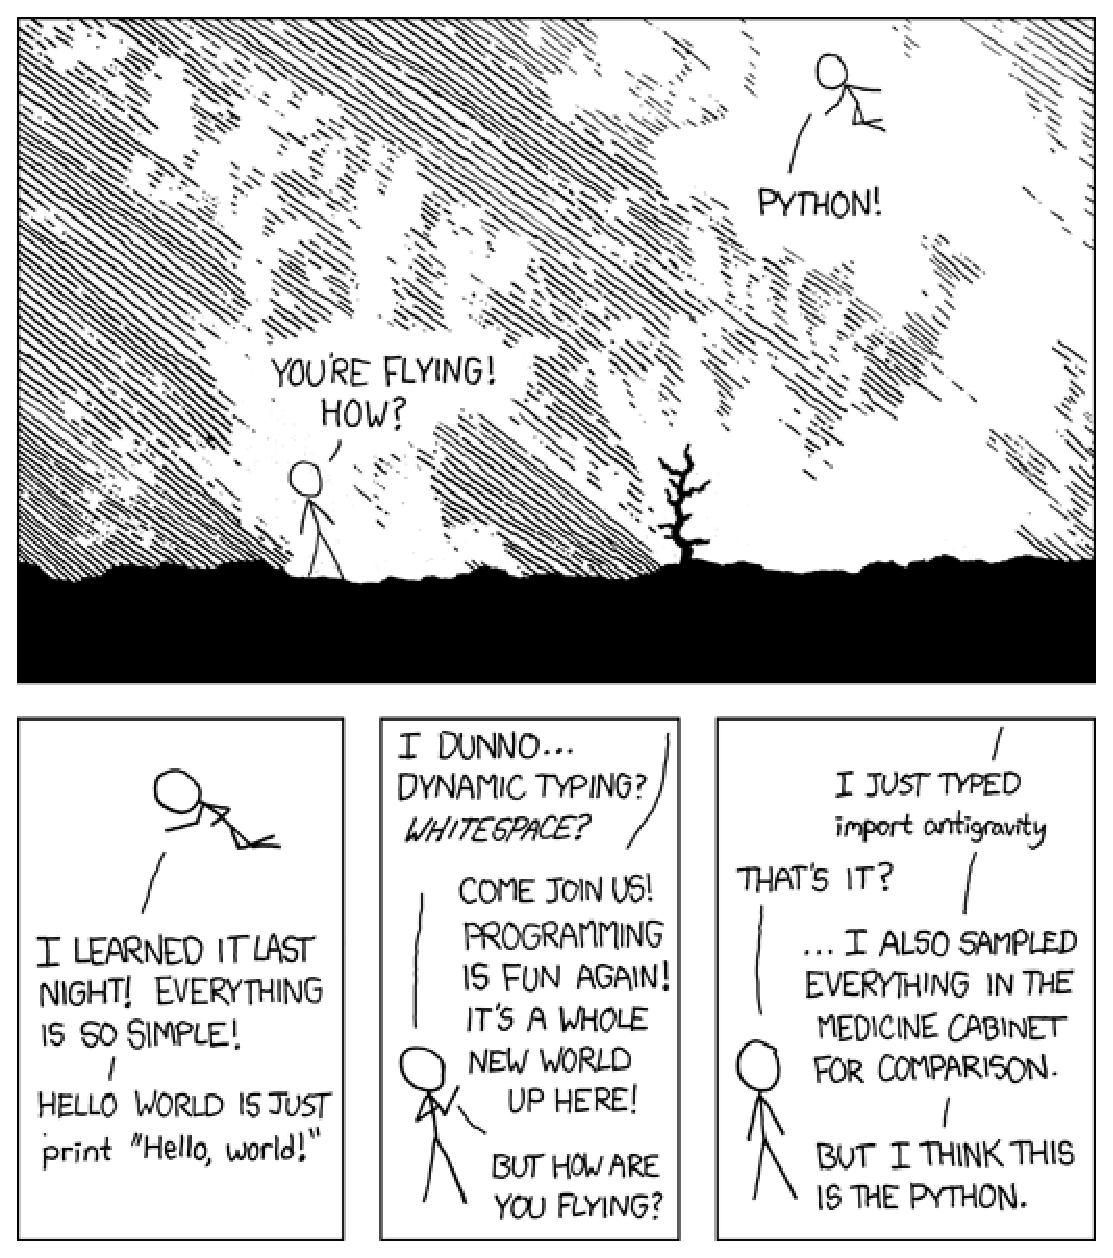
\includegraphics{python.eps}}
    \end{center}
  \end{frame}

%%%%%%%%%%%%%%%%%%%%%%%%%%%%%%%%%%%%%%%%%%%%%%%%%%%%%%%%%%%%%%%%%%%%%%%%%%%%%%

  \section{Interaktivní shell}
  \begin{frame}[t]
    \frametitle{Interaktivní shell}
    \begin{block}{Interaktivní shell}
      Python umožňuje spouštět příkazy v~interaktivním shellu. Pro spuštění
      Python shellu (v~unixovém operačním systému) slouží příkaz 
      \texttt{python} nebo pro Python verze 3 příkaz \texttt{python3}
    \end{block}
    \begin{exampleblock}{Ukázka}
      \pythonhello
    \end{exampleblock}
  \end{frame}
  \begin{frame}[t]
    \frametitle{Interaktivní shell}
    \begin{block}{Konfigurace shellu}
      \begin{itemize}
        \item Shell si lze přizpůsobit podobně jako \textbf{bash} aj. 
          konfiguračním souborem \textbf{.pythonrc.py}.
        \item V~prostředí ze kterého je Python spouštěn musí být nastavena
          proměnná \texttt{PYTHONSTARTUP} s~cestou ke konfiguračnímu souboru
        \item Ukázka konfiguračního souboru: 
          \myurl{
            https://github.com/whiteinge/dotfiles/blob/master/.pythonrc.py
          }
      \end{itemize}
    \end{block}
  \end{frame}

%%%%%%%%%%%%%%%%%%%%%%%%%%%%%%%%%%%%%%%%%%%%%%%%%%%%%%%%%%%%%%%%%%%%%%%%%%%%%%

  \section{PyPI}
  \begin{frame}[t]
    \frametitle{PyPI}
    \begin{block}{PyPI}
       \begin{itemize}
          \item \textbf{PyPI} -- \textbf{Py}thon \textbf{P}ackage 
            \textbf{I}ndex je repozitář s~balíčky třetích stran
          \item Umožňuje jednoduché přidávání nestandardních knihoven
          \item Instalace balíčků z~repozitáře příkazem \\
            \texttt{pip install <package>}
          \item Odstranění nainstalovaných balíčků příkazem \\
            \texttt{pip uninstall <package>}
        \end{itemize}
    \end{block}
  \end{frame}

%%%%%%%%%%%%%%%%%%%%%%%%%%%%%%%%%%%%%%%%%%%%%%%%%%%%%%%%%%%%%%%%%%%%%%%%%%%%%%

  \section{Ukázka použití Pythonu}
  \begin{frame}[t]
    \frametitle{Ukázka použití Pythonu}
    \begin{block}{Výpočet vzdálenosti bodů v~prostoru}
      Pro ukázku Pythonu bude použit výpočet vzdálenosti bodů v~prostoru
      pomocí vzorce
      \[|AB| = \sqrt{(b_{1} - a_{1})^{2} +
                     (b_{2} - a_{2})^{2} +
                     (b_{3} - a_{3})^{2}
                    }
      \]
    \end{block}
  \end{frame}
  \begin{frame}[t]
    \frametitle{Ukázka použití Pythonu}
    \begin{exampleblock}{Obsah souboru example.py}
      \pythonexample
    \end{exampleblock}
    \begin{exampleblock}{Spuštění z~interaktivního shellu}
      \pythonuseexample      
    \end{exampleblock}
  \end{frame}

%%%%%%%%%%%%%%%%%%%%%%%%%%%%%%%%%%%%%%%%%%%%%%%%%%%%%%%%%%%%%%%%%%%%%%%%%%%%%%

  \section{Použité zdroje}
  \begin{frame}[t]
    \frametitle{Použité zdroje}
    \begin{itemize}
      \item Wikipedia \\
        \myurl{
          https://en.wikipedia.org/wiki/Python\_\%28programming\_language\%29
        } 
      \item xkcd \\ \myurl{http://xkcd.com/353/}
      \item Dokumentace k~Python 2 \\ \myurl{https://docs.python.org/2/}
      \item Dokumentace k~Python 3 \\ \myurl{https://docs.python.org/3/}
      \item Python Package Index \\ \myurl{https://pypi.python.org/pypi}
      \item Seth House, repozitář GitHub \\ 
        \myurl{https://github.com/whiteinge/dotfiles}
    \end{itemize}
  \end{frame}

%%%%%%%%%%%%%%%%%%%%%%%%%%%%%%%%%%%%%%%%%%%%%%%%%%%%%%%%%%%%%%%%%%%%%%%%%%%%%%

\end{document}
